\documentclass[a4]{article}
\usepackage{a4wide}
\usepackage{amsmath}
\usepackage{amsfonts}
\usepackage{amssymb}
\usepackage{array}
\usepackage{multicol}
\usepackage{graphicx}
\usepackage{subfig}

\usepackage[pagebackref=true]{hyperref}

\begin{document}
\title{LO3 MAC Simulator}
\author{Murukesh Mohanan\\133059001}
\maketitle
\section{Compilation}
The code is reasonably organized: you can find the source files in \texttt{src/}, 
header files in \texttt{inc/}, object files and binaries in \texttt{obj/} and 
\texttt{bin/} respectively, and so on. Files related to this report are present 
in \texttt{doc/}. Simulation results for the most recent run are in
\texttt{tests/} and archived results in \texttt{archives/}. 
Compiling is simple:
\begin{itemize}
	\item To compile the normal binary, do \\
		\texttt{make [norm]}  \\
		This creates \texttt{bin/lo3mac}, which relies on a 
		pre-created \texttt{recordFlow.txt}.\\
		To run it, do: \\
		\texttt{bin/lo3mac} $\langle$error rate$\rangle$ 
			$\langle$sim duration$\rangle$
	\item To compile the generator binary, do \\
		\texttt{make gen} \\
		This creates \texttt{bin/gen\_lo3mac}, which generates 
		\texttt{recordFlow.txt} for future use.\\
		To run it do: \\
		\texttt{bin/gen\_lo3mac} $\langle$error rate$\rangle$ 
			$\langle$sim duration$\rangle$ $\langle$call interval$\rangle$
			$\langle$call duration$\rangle$ 
			$\langle$stored voice duration$\rangle$\footnote{Please refer to Table \ref{table:params} for details on these parameters.}
	\item To run the test simulation, do \\
		\texttt{make test}\\
		and then to update this document, do \\
		\texttt{make report}
\end{itemize}
For various reasons, I decided to let the default target of \texttt{make}
be \texttt{bin/lo3mac} instead of this report.
\section{Execution}
The \texttt{run\_tests.sh}, \texttt{parse\_output.sh} and 
\texttt{plot\_data.sh} are various helper scripts:
\begin{itemize}
	\item \texttt{run\_tests.sh} runs the simulator for various
	pre-set parameters, 
	\item \texttt{parse\_output.sh} sifts through the output of the
	simulator for the values we need, and 
	\item \texttt{plot\_data.sh} takes this data and runs various Python 
	scripts on them and finally plots them.
\end{itemize}
DO edit the shell scripts and change \texttt{\$PROJDIR} to reflect the 
absolute path of the project directory before running them. The Python
scripts in the badly-named \texttt{scripts} directory need not be 
modified.

\begin{table}[m]
\centering
\begin{tabular}{|l|r|l|m{'2cm'}}
	\hline
	Parameter & Range & Unit \\ \hline
	Error Rate & $[0, 1)$ & (probability) \\
	Simulation Duration & $(0, \infty$) & hours \\
	Inter-Call DUration & $[0, 3)$ & hours \\
	Call Duration & $[0, 4)$ & minutes \\
	Stored Voice Duration & $[0, 4)$ & minutes \\ \hline
\end{tabular}
\caption{Description of simulator parameters.}
\label{table:params}
\end{table}

\begin{figure}
\centering
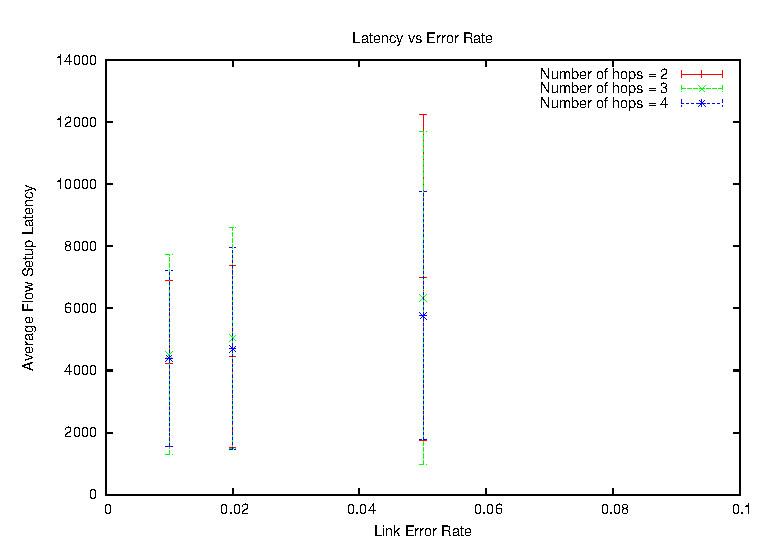
\includegraphics[width=0.9\textwidth]{latency-vs-error.eps}
\end{figure}
\begin{figure}
\centering
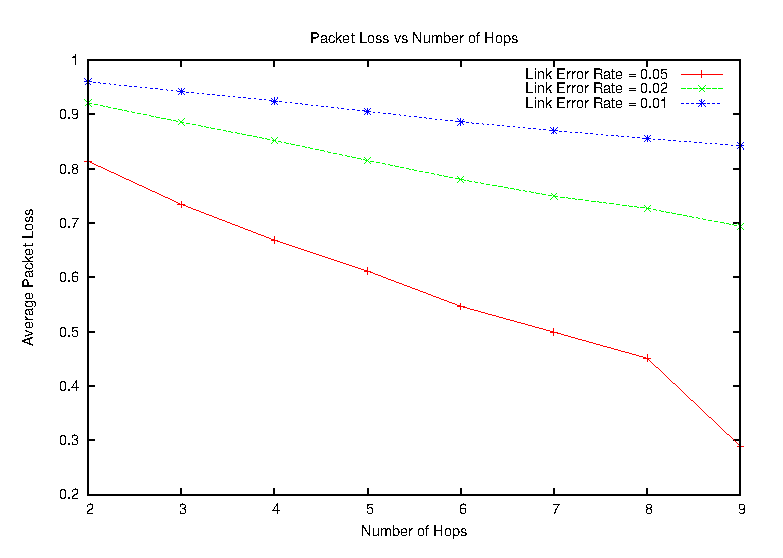
\includegraphics[width=0.9\textwidth]{loss-vs-hops.eps}
\end{figure}
\begin{figure}
\centering
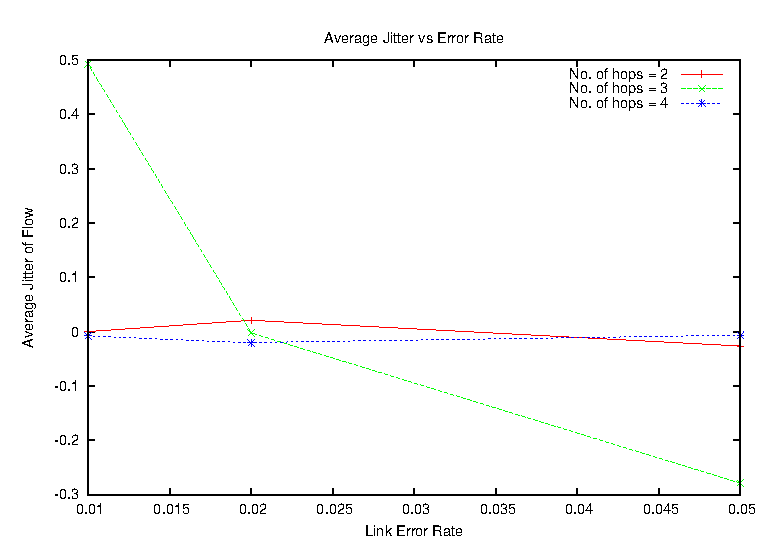
\includegraphics[width=0.9\textwidth]{jitter-vs-error.eps}
\end{figure}
\begin{figure}
\centering
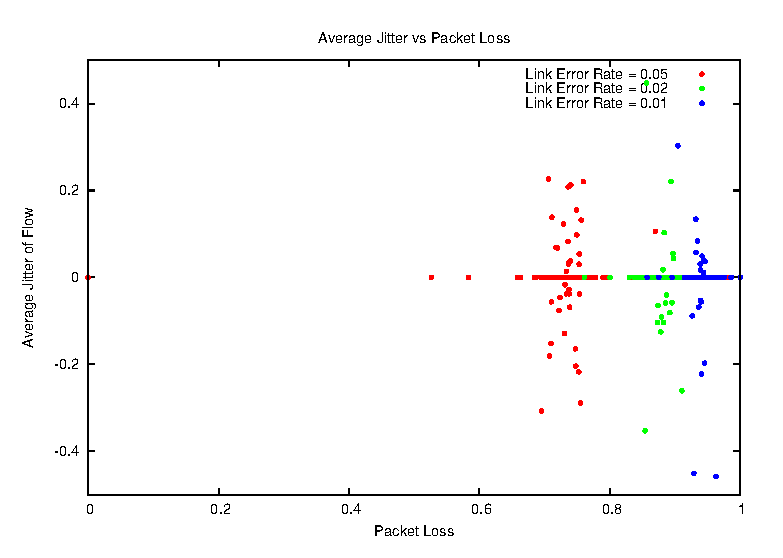
\includegraphics[width=0.9\textwidth]{jitter-vs-loss.eps}
\end{figure}
\begin{figure}
\centering
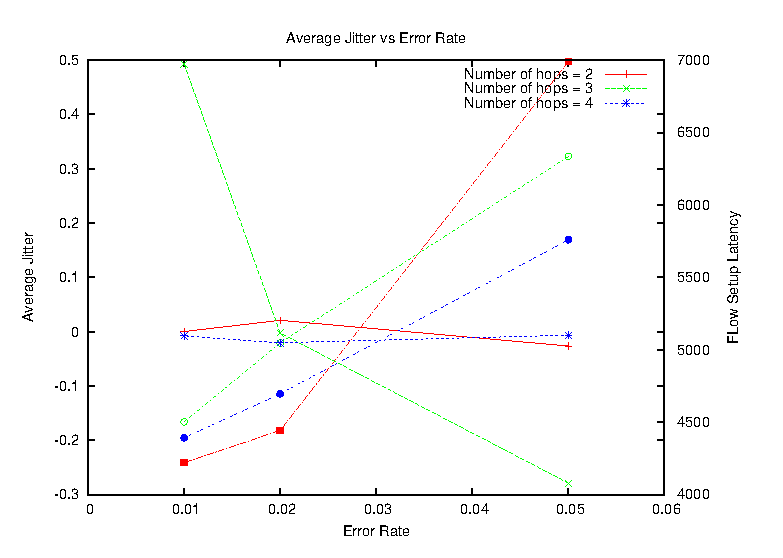
\includegraphics[width=0.9\textwidth]{jitter-latency-vs-error.eps}
\end{figure}

\end{document}

